\subsection{Vertical Translation}

Now the analogous alteration to the previous one will be analyzed, which is the vertical translation. \Fig~\ref{fig:acc_vt_wu} shows the alteration graphs for both networks. The behavior is very similar to the vertical alteration. The reason is again in the structural limits of network architecture.

\begin{figure}[h]
	\centering
	\begin{subfigure}{.5\textwidth}
		\centering
		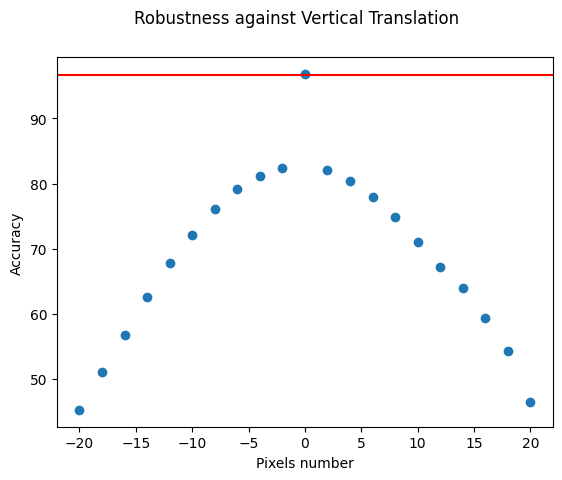
\includegraphics[width=0.8\linewidth]{ImageFiles/EvalBNN/VT/WU/acc}
		\caption{BNN}
		\label{fig:vt_acc_wu_bnn}
	\end{subfigure}%
	\begin{subfigure}{.5\textwidth}
		\centering
		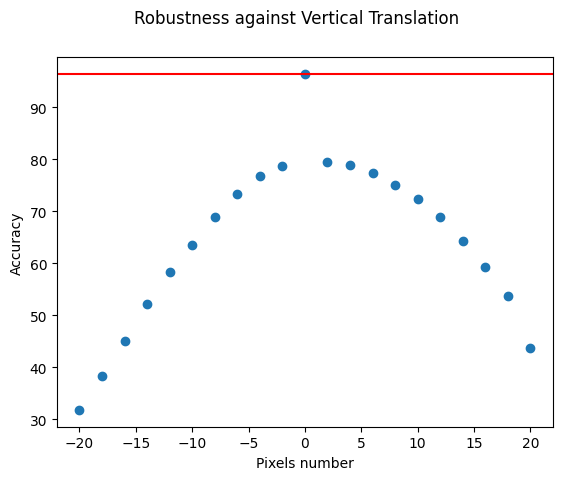
\includegraphics[width=0.8\linewidth]{ImageFiles/EvalANN/vert_trans_ann}
		\caption{Standard NN}
		\label{fig:vert_trans_ann}
	\end{subfigure}
	\caption{Accuracy trend for vertical translation}
	\label{fig:acc_vt_wu}
\end{figure}

The robustness metrics computed with this alteration are $0.8625$ for the BNN and $0.8412$ for the standard NN.

\Fig~\ref{fig:vt_uncertainty} illustrates the trend of the two uncertainties, which reflects again the accuracy trend in \Fig~\ref{fig:vt_acc_wu_bnn}.

\begin{figure}[h]
	\centering
	\begin{subfigure}{.5\textwidth}
		\centering
		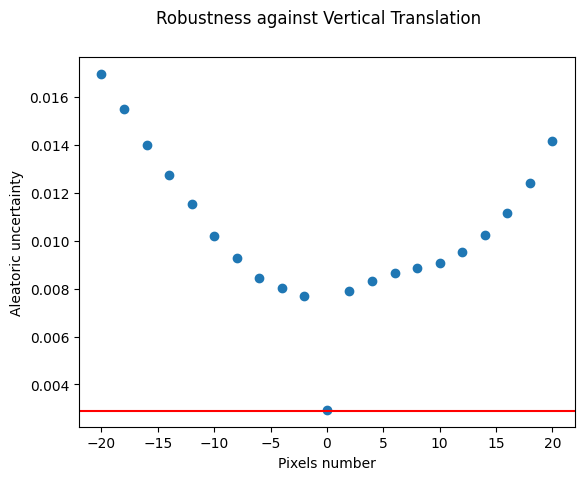
\includegraphics[width=0.8\linewidth]{ImageFiles/EvalBNN/VT/aleatoric}
		\caption{Aleatoric uncertainty}
		\label{fig:vt_aleatoric}
	\end{subfigure}%
	\begin{subfigure}{.5\textwidth}
		\centering
		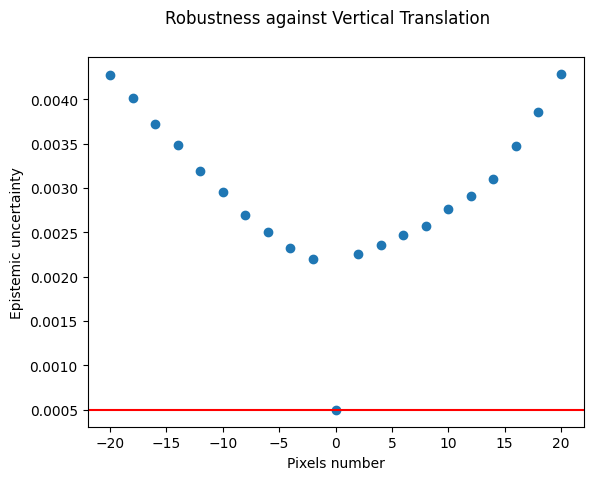
\includegraphics[width=0.8\linewidth]{ImageFiles/EvalBNN/VT/epistemic}
		\caption{Epistemic uncertainty}
		\label{fig:vt_epistemic}
	\end{subfigure}
	\caption{Uncertainty trend for vertical translation}
	\label{fig:vt_uncertainty}
\end{figure}

\vspace{0.3cm}
\textbf{Classification using aleatoric uncertainty}
\vspace{0.1cm}

As it is possible to see in \Fig~\ref{fig:vt_au}, the use of aleatoric uncertainty in the classification does not lead to substantial improvements in terms of robustness.

\begin{figure}[h]
	\centering
	\begin{subfigure}{.33\textwidth}
		\centering
		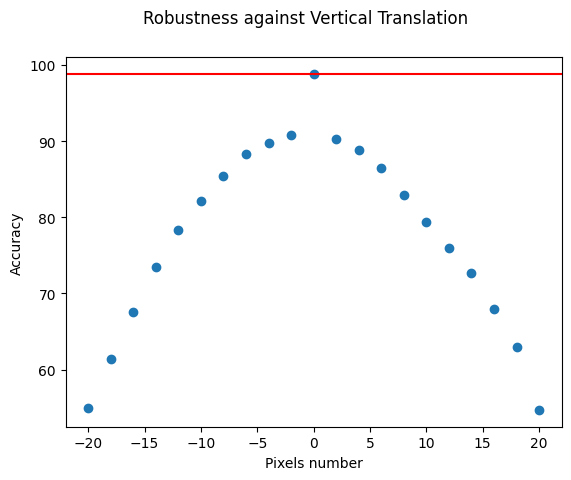
\includegraphics[width=0.9\linewidth]{ImageFiles/EvalBNN/VT/AU/acc}
		\caption{Accuracy using aleatoric \\ uncertainty}
		\label{fig:vt_au_acc}
	\end{subfigure}%
	\begin{subfigure}{.33\textwidth}
		\centering
		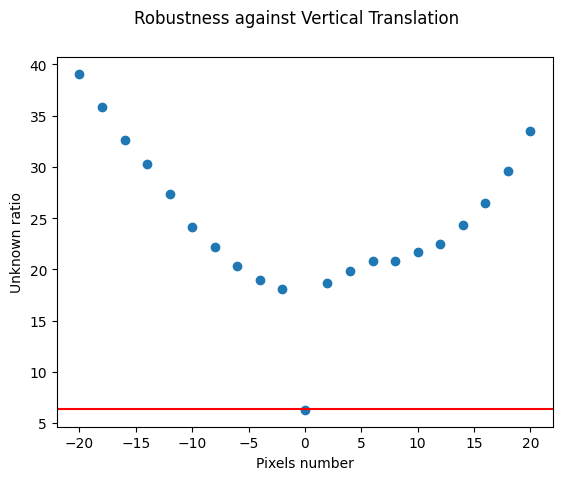
\includegraphics[width=0.9\linewidth]{ImageFiles/EvalBNN/VT/AU/unkn}
		\caption{Unknown ratio using aleatoric uncertainty}
		\label{fig:vt_au_unkn}
	\end{subfigure}%
	\begin{subfigure}{.33\textwidth}
		\centering
		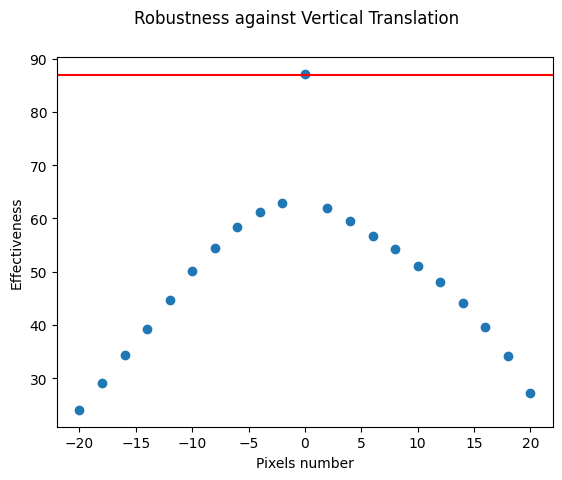
\includegraphics[width=0.9\linewidth]{ImageFiles/EvalBNN/VT/AU/eff}
		\caption{Effectiveness using aleatoric uncertainty}
		\label{fig:vt_au_eff}
	\end{subfigure}
	\caption{Robustness graph for vertical translation when aleatoric uncertainty is employed in the classification}
	\label{fig:vt_au}
\end{figure}

\Tab~\ref{table:rob_vt_au} indicates that the robustness in terms of accuracy increases, but the augmented robustness is very low due to the high unknown ratio reached.

\begin{table}[h]
	\centering
	\begin{tabular}{|| l | l ||} 
		\hline
		\textbf{Parameter} & \textbf{Value} \\
		\hline
		\hline
		$rob_{VerticalTranslation}$ & $0.8994$ \\
		$robInd_{VerticalTranslation}$ & $0.9065$ \\
		$robAug_{VerticalTranslation}$ & $0.7863$ \\	
		\hline
	\end{tabular}	
	\caption{Robustness metrics for the vertical translation when the aleatoric uncertainty is employed}
	\label{table:rob_vt_au}
\end{table}

\vspace{0.3cm}
\textbf{Classification using epistemic uncertainty}
\vspace{0.1cm}

The same analysis is conducted for the epistemic uncertainty and the results are shown in \Fig~\ref{fig:vt_eu}. The trends observed are the same as in the previous case.

\begin{figure}[h]
	\centering
	\begin{subfigure}{.33\textwidth}
		\centering
		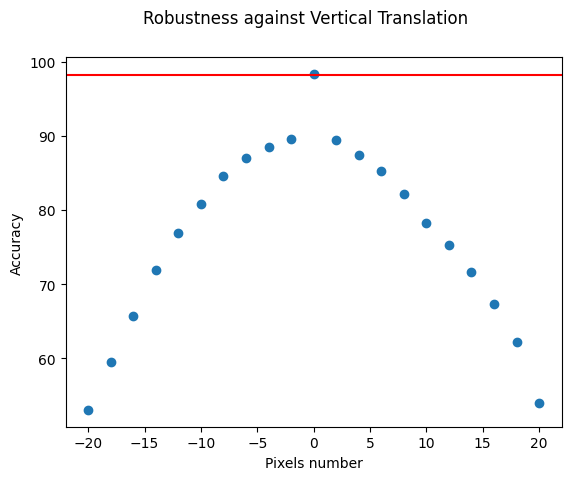
\includegraphics[width=0.9\linewidth]{ImageFiles/EvalBNN/VT/EU/acc}
		\caption{Accuracy using epistemic \\ uncertainty}
		\label{fig:vt_eu_acc}
	\end{subfigure}%
	\begin{subfigure}{.33\textwidth}
		\centering
		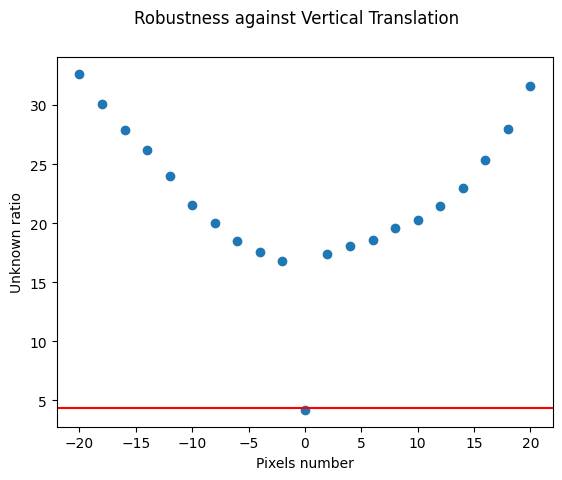
\includegraphics[width=0.9\linewidth]{ImageFiles/EvalBNN/VT/EU/unkn}
		\caption{Unknown ratio using \\ epistemic uncertainty}
		\label{fig:vt_eu_unkn}
	\end{subfigure}%
	\begin{subfigure}{.33\textwidth}
		\centering
		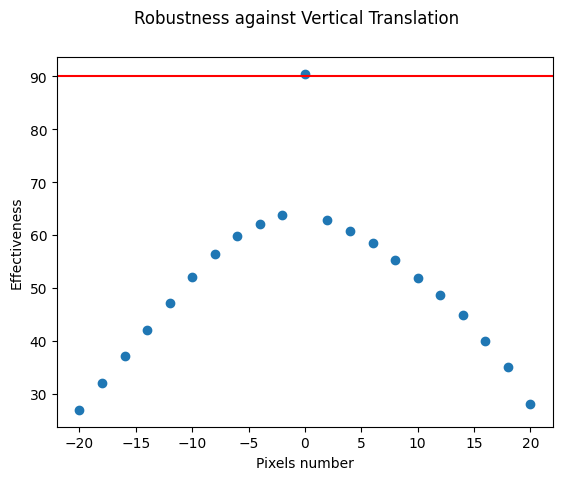
\includegraphics[width=0.9\linewidth]{ImageFiles/EvalBNN/VT/EU/eff}
		\caption{Effectiveness using \\ epistemic uncertainty}
		\label{fig:vt_eu_eff}
	\end{subfigure}
	\caption{Robustness graph for vertical translation when epistemic uncertainty is employed in the classification}
	\label{fig:vt_eu}
\end{figure}

\Tab~\ref{table:rob_vt_eu} displays the robustness metrics calculated through the utilization of epistemic uncertainty within the classification procedure. The results obtained resemble those from the previous scenario, which confirms the network inherent structural limitations.

\begin{table}[h]
	\centering
	\begin{tabular}{|| l | l ||} 
		\hline
		\textbf{Parameter} & \textbf{Value} \\
		\hline
		\hline
		$rob_{VerticalTranslation}$ & $0.8957$ \\
		$robInd_{VerticalTranslation}$ & $0.9102$ \\
		$robAug_{VerticalTranslation}$ & $0.7854$ \\	
		\hline
	\end{tabular}	
	\caption{Robustness metrics for the vertical translation when the epistemic uncertainty is employed}
	\label{table:rob_vt_eu}
\end{table}

\vspace{0.3cm}
\textbf{Classification using standard deviation}
\vspace{0.1cm}

The outcomes when employing standard deviation, as illustrated in \Fig~\ref{fig:vt_vu}, do not significantly enhance performance as in the previous cases.

\begin{figure}[h]
	\centering
	\begin{subfigure}{.33\textwidth}
		\centering
		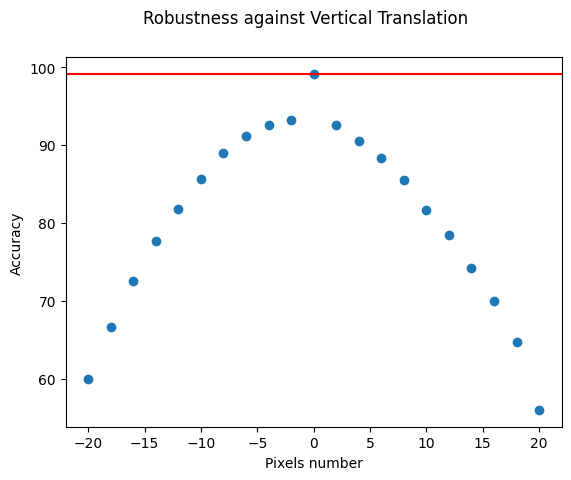
\includegraphics[width=0.9\linewidth]{ImageFiles/EvalBNN/VT/VU/acc}
		\caption{Accuracy using standard \\ deviation}
		\label{fig:vt_vu_acc}
	\end{subfigure}%
	\begin{subfigure}{.33\textwidth}
		\centering
		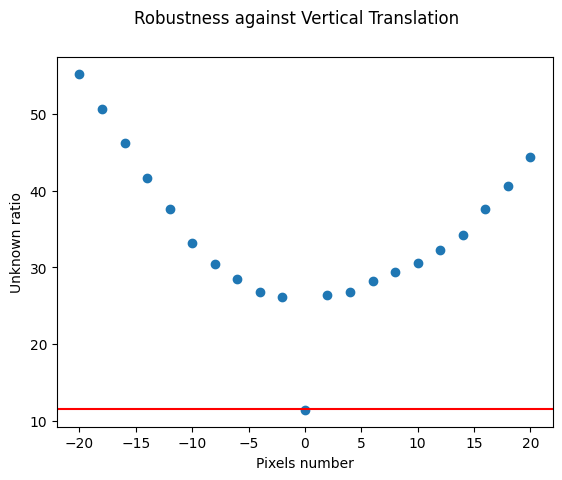
\includegraphics[width=0.9\linewidth]{ImageFiles/EvalBNN/VT/VU/unkn}
		\caption{Unknown ratio using \\ standard deviation}
		\label{fig:vt_vu_unkn}
	\end{subfigure}%
	\begin{subfigure}{.33\textwidth}
		\centering
		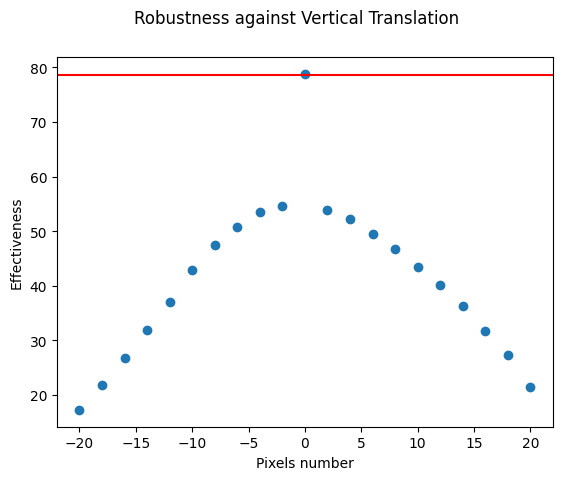
\includegraphics[width=0.9\linewidth]{ImageFiles/EvalBNN/VT/VU/eff}
		\caption{Effectiveness using standard deviation}
		\label{fig:vt_vu_eff}
	\end{subfigure}
	\caption{Robustness graph for vertical translation when standard deviation is employed in the classification}
	\label{fig:vt_vu}
\end{figure}

\Tab~\ref{table:rob_vt_vu} gives the quantitative robustness measurements. The $rob$ metric is higher in this case, the reason is due to the pessimistic behavior obtained using standard deviation as uncertainty measure.

\begin{table}[h]
	\centering
	\begin{tabular}{|| l | l ||} 
		\hline
		\textbf{Parameter} & \textbf{Value} \\
		\hline
		\hline
		$rob_{VerticalTranslation}$ & $0.9120$ \\
		$robInd_{VerticalTranslation}$ & $0.8764$ \\
		$robAug_{VerticalTranslation}$ & $0.7693$ \\	
		\hline
	\end{tabular}	
	\caption{Robustness metrics for the vertical translation when the standard deviation is employed}
	\label{table:rob_vt_vu}
\end{table}

\vspace{0.3cm}
\textbf{Comparison}
\vspace{0.1cm}

The results summary of this analysis is presented in \Tab~\ref{table:rob_vt}. It is evident that the network exhibits slightly better robustness to vertical translation compared to horizontal translation. However, the overall performance remains poor, and the utilization of uncertainty in this context does not appear to be effective. To address this issue, employing a Bayesian CNN may be a potential solution.

\begin{table}[H]
	\centering
	\begin{tabular}{|| l | l | l | l ||} 
		\hline
		\textbf{Parameter} & \textbf{Aleatoric} & \textbf{Epistemic} & \textbf{Standard deviation} \\
		\hline
		\hline
		$rob_{VerticalTranslation}$ & $0.8994$ & $0.8957$ & $0.9120$ \\
		$robInd_{VerticalTranslation}$ & $0.9065$ & $0.9102$ & $0.8764$ \\
		$robAug_{VerticalTranslation}$ & $0.7863$ & $0.7854$ & $0.7693$ \\	
		\hline
	\end{tabular}	
	\caption{Summary of the robustness metrics for the vertical translation}
	\label{table:rob_vt}
\end{table}